\documentclass[11pt]{article}
% Self-contained NMI-style preamble (standard TeX Live packages only).
\usepackage[margin=1in]{geometry}
\usepackage{graphicx}
\usepackage{amsmath}
\usepackage{booktabs}
\usepackage{siunitx}
\usepackage{caption}
\usepackage[hidelinks]{hyperref}
\usepackage[round]{natbib}
\usepackage{xcolor}
\captionsetup{labelfont=bf,font=small,labelsep=period}
\newcommand{\figbar}[1]{\textbf{Fig.~#1~$\vert$}}
\setlength{\parskip}{2pt}
\title{\vspace{-2em}\textbf{A Socratic council operationalizes vague research questions into
falsifiable, instrument-testable hypotheses}}
\author{\normalsize [Authors]\\[-0.3em]\normalsize [Affiliations]}
\date{}

\begin{document}
\maketitle
\vspace{-2em}

\begin{abstract}
\noindent Autonomous ``AI scientist'' systems can generate ideas and run experiments, but they treat hypothesis
\emph{formulation} as a single generative step and optimize for novelty rather than testability---so their
hypotheses are often novel-sounding yet not operationalized against any specific instrument. We introduce the
\textbf{Socratic Council}, a multi-agent architecture that makes the philosophy of science executable and
performs the missing \emph{operationalization} stage: a maieutic \emph{proposer} (abduction), an elenctic
\emph{skeptic} (Socratic ignorance), and a rubric-bound \emph{judge} debate a vague question into a falsifiable,
discriminating, instrument-testable hypothesis, terminating on a falsifiability criterion rather than on
agreement. Evaluated on ten literature-grounded questions in single-cell \emph{E. coli} biology against a
whole-cell simulator, the dialectic does not change how \emph{testable} hypotheses \emph{look}---a coarse
operationalization-quality rubric saturates for every configuration---but it makes them measurably
\emph{sounder}: a fresh, configuration-blind, cross-family auditor finds the full Council leaves
$\sim$20\% fewer substantive methodological defects than a single strong prompt or a critic-free ablation
(paired one-sided Wilcoxon $p=0.001$), with the reduction largest on the hardest-to-operationalize questions and
the elenctic \emph{skeptic} identified as the active ingredient. A first-class \texttt{Hypothesis} object carries
an executable falsifier that we run against fresh simulations to return confirm/refute verdicts. An information
quarantine---an import-level control that denies the Council the answer key---ensures the metric measures
\emph{derivation}, not recall. We argue that a disciplined operationalization stage, held to a
philosophy-of-science rubric, is a missing and separable component of AI-driven scientific reasoning.
\end{abstract}

\section{Introduction}
A whole-cell simulator or a robotic laboratory can, in principle, test almost any single-cell hypothesis---but
only once the hypothesis is stated \emph{testably}. Users arrive with questions such as ``do genetically
identical cells behave differently?'', which name no observable, no baseline, no prediction and no refuting
result. Turning such a question into a falsifiable claim is the step that philosophy of science calls
\emph{operationalization} \citep{bridgman1927logic} within Reichenbach's \emph{context of discovery}
\citep{reichenbach1938experience}, and it is precisely the step current AI-scientist systems skip.

The dominant systems---Sakana's AI Scientist \citep{lu2024aiscientist,yamada2025aiscientistv2}, Google's AI
co-scientist \citep{gottweis2025coscientist}, autonomous chemistry agents \citep{boiko2023coscientist}, the
Robot Scientists \citep{king2004robotscientist,king2009automation}, and virtual/agent laboratories
\citep{swanson2024virtuallab}---automate the loop from ideation to experiment, but treat hypothesis formulation
as a lightweight prompt and optimize downstream signals: perceived novelty, or an Elo tournament of expert
preference. A large blinded study finds LLM-generated ideas are rated \emph{more novel but less feasible} than
expert ideas \citep{si2024llmideas}; ideation systems explicitly optimize novelty \citep{wang2024scimon}. None
imposes an explicit constraint that a hypothesis be \emph{operationalized against a named instrument's
measurable capabilities}, be falsifiable in the sense of \citet{popper1959logic} and \citet{platt1964strong},
and be produced under conditions that prevent the answer from leaking into its own formulation.

Multi-agent debate improves factuality and reasoning \citep{du2023debate,irving2018debate}, and rubric-bound
self-critique is established \citep{bai2022constitutional,madaan2023selfrefine,shinn2023reflexion}; but these
optimize \emph{answer correctness}, not the epistemic quality of a \emph{hypothesis}, and terminate on
agreement rather than on falsifiability. We ask whether a dialectic that instantiates the norms of the
philosophy of science---abduction, falsifiability, operationalism, strong inference, multiple working
hypotheses \citep{chamberlin1890multiple}, and the Duhem--Quine belt of auxiliary assumptions
\citep{quine1951dogmas}---can perform this missing operationalization stage, and whether doing so measurably
improves the hypotheses over a single strong prompt.

\paragraph{Contributions.} (i) The \textbf{Socratic Council}, a proposer/skeptic/judge architecture that
computes the discovery$\to$operationalization$\to$justification arc and terminates on a falsifiability gate.
(ii) A pre-registered evaluation on ten literature-grounded questions showing that the dialectic's value is
\emph{not} visible on a coarse quality rubric (which saturates) but is significant and cross-family-replicated
on a sensitive residual-defect metric, with the elenctic skeptic as the active ingredient. (iii) A first-class
executable \texttt{Hypothesis} object and a verdict engine that runs the Council's own falsifiers against fresh
whole-cell simulations. (iv) An \textbf{information quarantine}: an auditable, import-level control that ensures
the system \emph{derives} rather than \emph{recalls} operationalizations.

\section{Results}

\begin{figure}[t]
\centering
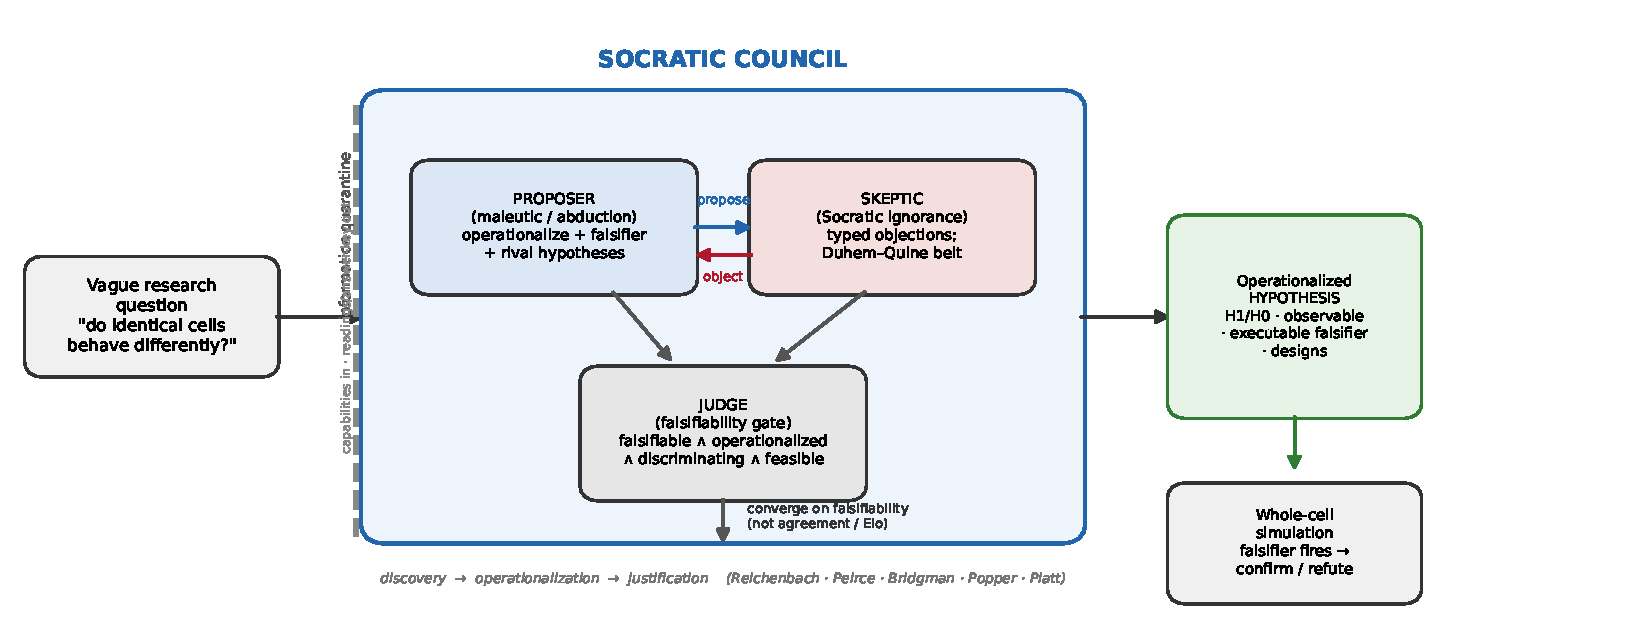
\includegraphics[width=\textwidth]{figures/fig1_architecture.pdf}
\caption{\figbar{1} \textbf{The Socratic Council.} A vague question is transformed by a proposer (maieutic
abduction), an elenctic skeptic (Socratic ignorance), and a rubric-bound judge that converges on falsifiability
rather than agreement, yielding a first-class operationalized \texttt{Hypothesis} whose executable falsifier is
run against a whole-cell simulation. The Council operates behind an \emph{information quarantine}: it sees the
instrument's measurable capabilities but never its readings or the literature answer key. The three roles
compute Reichenbach's discovery$\to$justification arc via the middle bridge of operationalization.}
\end{figure}

\subsection{The Socratic Council}
The Council (Fig.~1) transforms a question through three roles, each an epistemic stance. The
\textbf{maieutic proposer} performs abduction: it emits the sharpest candidate hypothesis, operationalizing every
construct onto a real instrument observable (Bridgman), with a predicted effect, a falsifier (a risky
prohibition that could fail; Popper), and at least two rival hypotheses each with a distinguishing experiment
(Chamberlin/Platt). The \textbf{elenctic skeptic} adopts Socratic ignorance: it raises typed objections
(undefined term, hidden Duhem--Quine auxiliary, unfalsifiable claim, rival-not-excluded, or a claim that
outruns the instrument). The \textbf{rubric-bound judge} is a gate, not a scorer: it certifies a hypothesis only
when it is falsifiable, specified, operationalized onto real observables with a named statistical test, and
discriminating, and terminates on this falsifiability criterion together with a convergence signal---never on
mere agreement, novelty, or Elo. The output is a first-class \texttt{Hypothesis} object: H$_1$/H$_0$,
operational definitions bound to observables, an executable falsifier, rival hypotheses, the auxiliary-assumption
belt, and envelope-checked candidate experimental designs.

A worked trace on the flagship question ``do genetically identical \emph{E. coli} cells behave differently?''
illustrates the mechanism. The proposer produces a hypothesis (isogenic cells show phenotypic heterogeneity,
coefficient of variation $\geq 0.15$ across replicate seeds, driven by stochastic gene expression) with a
CV-based falsifier and three rivals. In a second round the skeptic identifies two \emph{substantive} defects a
single-shot prompt would have shipped: a control design that ``outruns the instrument'' (it presumes a
perturbation can suppress variance when it can only shift the mean), and a rival-discrimination prediction that
is internally \emph{contradictory}. The proposer repairs both---replacing the infeasible control, clarifying the
mechanism, and adding a second knockout as a discriminating arm---after which the judge certifies convergence.
The dialectic thus improves the \emph{experimental design}, not merely the prose.

\subsection{The dialectic makes hypotheses sounder, not more testable-looking}
We evaluated four configurations---\textbf{full} (proposer+skeptic+judge), \textbf{no\_skeptic}
(proposer+judge), \textbf{proposer\_only} (single-shot generation, the baseline), and \textbf{generic\_judge}
(proposer+skeptic with a plain quality judge, no falsifiability rubric)---on ten literature-grounded questions
(three replicates each; Claude Sonnet 4.5 roles at temperature 0.7). Two metrics were pre-registered:
a six-criterion operationalization-quality rubric graded blind to the literature answer, and---after observing
the rubric saturate on the first cases, and before the full audit was read---a more sensitive
\emph{residual-defect} count from a fresh adversarial auditor blind to configuration. Both metrics were scored
by an independent Claude judge \emph{and} a cross-family GPT-4o judge.

The binary quality rubric is a clean \textbf{null} (Fig.~2C): every configuration scores $\approx 6/6$ (full and
proposer\_only both $6.0$; Claude--GPT mean absolute score difference $0.017$). A single strong proposer already
writes \emph{formally} adequate hypotheses; the dialectic does not change how testable they \emph{look}.

On the sensitive metric, the full Council leaves \textbf{fewer substantive methodological defects} than the
baselines (Fig.~2A). On the cross-family GPT auditor, the full Council averages $3.80$ defects versus $4.77$ for
single-shot and $4.67$ for no\_skeptic---a $\sim$20\% reduction, significant under a one-sided paired Wilcoxon
signed-rank test across the ten cases ($p=0.001$ for both comparisons). The independent Claude auditor agrees in
direction ($3.37$ vs $4.50$ and $4.83$, a $\sim$25\% reduction) though with wider case-to-case variance and
without significance. The reduction is \textbf{largest on the hardest-to-operationalize questions} (Fig.~2B):
$2.0$ fewer defects on the flagship heterogeneity question and $1.3$ on non-genetic individuality, versus
$\approx 0.3$ on well-trodden ppGpp physiology where a single prompt already suffices. Every one of the ten
cases favours the full Council, which is why the paired test is significant despite modest per-case effects.

\begin{figure}[t]
\centering
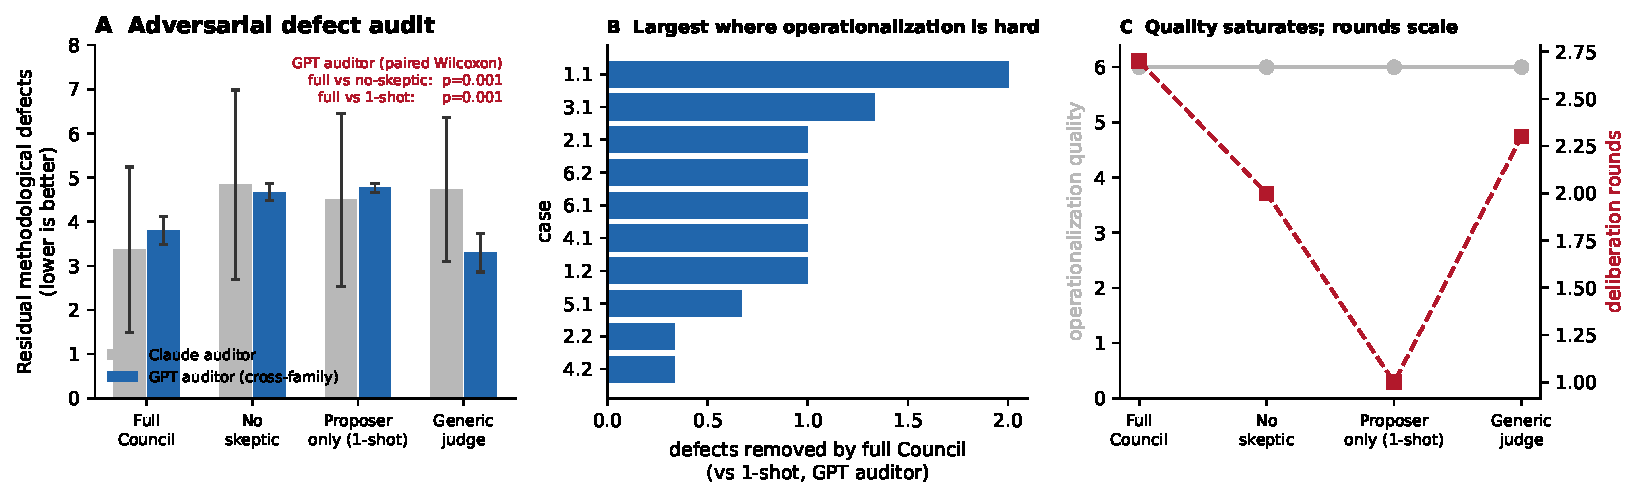
\includegraphics[width=\textwidth]{figures/fig2_mechanism.pdf}
\caption{\figbar{2} \textbf{The Socratic dialectic makes hypotheses sounder, not more testable-looking.}
\textbf{A}, Residual methodological defects per configuration, counted by a configuration-blind adversarial
auditor (grey: Claude Opus~4.8; blue: cross-family GPT-4o); error bars are 95\% case-clustered confidence
intervals. The full Council leaves fewer defects than the critic-free ablation and the single-shot baseline
(cross-family auditor, one-sided paired Wilcoxon, $p=0.001$). \textbf{B}, Per-case reduction of the full Council
versus single-shot (cross-family auditor); the effect is largest on the questions hardest to operationalize
(1.1 isogenic heterogeneity; 3.1 non-genetic individuality) and smallest on well-trodden physiology (4.2 ppGpp).
Every case favours the full Council. \textbf{C}, The two supporting signals: the binary operationalization-quality
rubric saturates (grey, a null---the dialectic does not change how testable hypotheses look) while deliberation
rounds scale with the dialectic (red). $n=3$ replicates $\times$ 10 cases per configuration.}
\end{figure}

\subsection{The elenctic skeptic is the active ingredient}
Component isolation localizes the effect to the critic rather than the rubric. \texttt{generic\_judge}, which
retains the skeptic but discards the falsifiability rubric, matches the full Council on the cross-family defect
metric ($3.30$ vs $3.80$), whereas \texttt{no\_skeptic} is clearly worse ($4.67$). Deliberation depth scales
correspondingly (Fig.~2C): mean rounds are $2.7$ (full), $2.3$ (generic\_judge), $2.0$ (no\_skeptic) and $1.0$
(single-shot). The dialectic's cost is more deliberation; its benefit is the removal of methodological
defects a single pass leaves behind.

\subsection{The hypotheses are instrument-testable}
The \texttt{Hypothesis} object's falsifier is executable. A verdict engine compiles it into a structured test
(the statistic, channel, target and reference designs, and threshold) and runs the actual statistic on per-seed
whole-cell simulation output, returning a confirm/refute verdict with a severity assessment against a
pre-registered smallest effect size of interest---not post-hoc power \citep{mayo2018severe}. On the flagship
question, executed against $n=16$ real isogenic simulations, the across-seed coefficient of variation is $0.066$
for growth rate (H$_1$ refuted, below the $0.10$ threshold), $0.013$ for ribosome concentration (refuted), and
$0.112$ for ppGpp concentration (supported, exceeding the effect-size floor). The loop closes: a vague question
becomes an operationalized hypothesis, whose falsifier fires on fresh simulation output and returns a verdict.

We stress the epistemic scope (Sec.~4): a verdict against a whole-cell model is a claim about the \emph{model},
which was itself fit to much of this literature \citep{macklin2020ecoli,oreskes1994verification}; for the
in-canon questions the loop is best read as \emph{blinded rediscovery / operationalization validation}, not
empirical confirmation \citep{winsberg2010simulation}.

\subsection{The quarantine measures derivation, not recall}
Because the proposer is a large language model that has read this literature, the evaluation must distinguish a
\emph{derived} operationalization from a \emph{recalled} answer. We enforce this with an \textbf{information
quarantine}: the module exposing the instrument to the Council is an import-level boundary that provides the
instrument's measurable capabilities (channel names, the runnable-perturbation vocabulary) but never its
readings or the literature answer key, and is statically prevented from importing any result-bearing code. In
scoping this control we found a real leak---a corpus statistic embedded in a tool's textual description---which
the boundary now excludes; the quarantine is thus an auditable engineering control against evaluation
contamination, of independent interest for closed-loop AI-science systems.

A leaked-versus-quarantined ablation (the proposer additionally handed each case's canonical answer; $n=3$
replicates $\times$ 10 cases, both auditors) shows what leakage actually changes. It does \emph{not} consistently
improve methodological soundness: the residual-defect count moves in opposite directions under the two auditors
(Claude $2.8$ leaked vs $4.7$ quarantined; GPT $4.1$ vs $3.3$). What it changes is \emph{recitation of measured
values the model would otherwise not assert}. The clearest case is essentiality (5.1), whose canonical answer is a
specific count ($\sim$300--620 essential genes): the leaked Council recites that count in $2/3$ runs, whereas the
quarantined Council recites it in $0/3$, proposing instead a \emph{falsifiable fraction} to test. Where the value
is derivable or textbook-familiar (the well-known five-fold ppGpp rise, 4.2), both recite it and the quarantine
neither can nor should matter. A benchmark scoring ``matches the literature'' can thus be inflated by recitation,
which the quarantine---by construction---prevents; our operationalization-quality metric is therefore an honest
measure of derivation. Whether leakage additionally drives a \emph{wrong} downstream conclusion on fresh
simulations, rather than mere recitation, requires executing the leaked hypotheses through the verdict engine and
is left to future work.

\section{Discussion}
Our central finding is deflationary in a useful way: a philosophy-of-science dialectic does not make an LLM's
hypotheses \emph{appear} more testable---on a coarse rubric, a single strong prompt already writes falsifiable,
discriminating hypotheses---but it makes them \emph{sounder}, removing substantive methodological defects that a
single pass leaves behind, most where operationalization is hardest, with the elenctic critique as the active
ingredient. This is a claim about \emph{operationalization}, a component that current AI-scientist systems
subsume into a novelty-optimizing ideation step. Isolated and held to a rubric, it is separately improvable and
separately measurable.

Two limitations bound the claims. First, evaluation is by LLM judges; we mitigate with a configuration-blind
adversarial auditor, a cross-family replication (the significant result is on the non-Claude auditor), and an
answer-key quarantine, but human-expert validation and additional families remain necessary. Second, the
instrument is a single simulator fit to the canon: in-canon closed-loop verdicts are rediscovery, not
confirmation, and only a pre-registered out-of-canon or wet-lab test would license a discovery claim. Finally,
we resist the temptation to over-read the Socratic framing: the skeptic checks the candidate against an external
rubric rather than deriving a contradiction from the interlocutor's own commitments, so the elenchus is an
organizing analogy \citep{vlastos1983elenchus} whose value we establish empirically, not by etymology.

The transferable message for autonomous science is that operationalization deserves to be a first-class,
instrumented stage---with a falsifiability-based termination criterion and an information quarantine---rather
than a side effect of ideation. A hypothesis that is novel but not operationalized cannot be tested; the
Council is a step toward closing that gap.

\section{Methods}
\paragraph{The Council.} Roles are large-language-model calls with forced-tool structured outputs
(Claude Sonnet 4.5, temperature 0.7). The judge applies a conjunctive gate over
\{falsifiable, specified, operationalized, discriminating, feasible\}; feasibility is computed deterministically
by checking each candidate design against the simulator's validated-perturbation envelope and a biosecurity
screen. Termination requires a clean judge certification plus a convergence signal (no new substantive
objection, or two stably-clean rounds); the operative early-exit is stability, not a fixed quota. On an
irreducible construct ambiguity the Council queries the user.

\paragraph{Instrument and quarantine.} The substrate is the public Covert-lab whole-cell \emph{E. coli} model
\citep{macklin2020ecoli}; the Council sees only a capability adapter (summary-channel names and units, species
kinds, the validated-perturbation vocabulary, the reference design, and the falsification mechanism) that
imports no result-bearing module and reads nothing under the data directory. A unit-test asserts the boundary.

\paragraph{Evaluation.} Ten questions span intrinsic/extrinsic noise, persistence, bet-hedging, non-genetic
individuality, growth laws, the stringent response, essentiality and diauxie, each with a canonical answer,
excluded rivals, and a wcEcoli observable mapping (Extended Data). The operationalization-quality rubric has six
answer-independent criteria; the residual-defect audit counts substantive methodological defects
(falsifier-cannot-fail, rival-not-discriminating, internal contradiction, infeasible design, unstated auxiliary,
vague construct, under-scoped) found by an auditor blind to configuration. Each hypothesis is graded by an
independent Claude (Opus 4.8) judge and a cross-family GPT-4o judge. The primary comparison is the full Council
versus single-shot on the case-clustered mean defect count (mean over three replicates within a case, then
across ten cases), by one-sided paired Wilcoxon signed-rank; convergence and feasibility rates use Wilson
intervals. Sampling temperature is pinned for the Council roles (the named variance source); reasoning-model
graders run at their defaults. Pre-registration (endpoints, rubric, per-case severity thresholds) is committed
before the confirmatory results were read.

\paragraph{Verdict engine.} A falsifier is compiled into a structured spec and executed on per-seed simulation
output: for a dispersion test, the across-seed coefficient of variation against an absolute threshold (the
simulator is seed-deterministic, so there is no same-seed technical-noise null); for a difference test, a Welch
$t$ on design means. Verdicts are scored target-versus-reference from the runs, not against the pooled corpus.
Severity is reported as whether the executed effect exceeds a pre-registered smallest effect size of interest.

\paragraph{Data and code availability.} All code, the ten-case benchmark, the pre-registration, and every result
JSON are in the project repository; figures regenerate from the committed result files.

\section*{Extended Data}
\begin{table}[h]
\centering\small
\caption{\textbf{Ablation summary} ($n=3$ replicates $\times$ 10 cases per configuration). Operationalization
quality is on a 0--6 scale (GPT auditor; the rubric saturates). Residual defects are lower-is-better (both
auditors). Convergence and feasibility are rates.}
\begin{tabular}{lccccc}
\toprule
Configuration & Quality (0--6) & Defects (GPT) & Defects (Claude) & Convergence & Mean rounds\\
\midrule
Full Council & 6.0 & \textbf{3.8} & \textbf{3.4} & 0.90 & 2.7\\
No skeptic & 6.0 & 4.7 & 4.8 & 1.00 & 2.0\\
Proposer only (1-shot) & 6.0 & 4.8 & 4.5 & 1.00 & 1.0\\
Generic judge & 6.0 & 3.3 & 4.7 & 0.90 & 2.3\\
\bottomrule
\end{tabular}
\end{table}

\begin{table}[h]
\centering\small
\caption{\textbf{Per-case defect reduction} of the full Council versus single-shot (cross-family GPT auditor).
Every case favours the full Council; the reduction is largest where operationalization is hardest.}
\begin{tabular}{llc}
\toprule
Case & Theme & Defects removed by full Council\\
\midrule
1.1 & isogenic gene-expression heterogeneity & 2.0\\
3.1 & non-genetic individuality & 1.3\\
1.2, 2.1, 4.1, 6.1, 6.2 & noise/persistence/growth-law/diauxie & 1.0\\
5.1 & knockout essentiality & 0.7\\
4.2, 2.2 & ppGpp stringent response; bet-hedging & 0.3\\
\bottomrule
\end{tabular}
\end{table}

\noindent The ten benchmark questions span intrinsic/extrinsic noise (1.1, 1.2), persistence and bet-hedging
(2.1, 2.2), non-genetic individuality (3.1), growth laws and the stringent response (4.1, 4.2), knockout
essentiality (5.1), and diauxie (6.1, 6.2); each carries a canonical answer, the rival hypotheses the seminal
work excluded, and a whole-cell observable mapping (full specification and every per-case operationalized
hypothesis are in the repository).

\small
\bibliographystyle{unsrtnat}
\bibliography{references}
\end{document}
